%  SingleXBs
%  Created by Dave Williams on 2009-06-25.
%  Copyright (c) 2009. All rights reserved.

% headder (fold)
\documentclass[]{article}

\usepackage{setspace, float, fancyhdr}
\usepackage[pdftex]{graphicx}
\usepackage[utf8]{inputenc}
\usepackage[round,numbers,sort&compress]{natbib} 
\addtolength{\parskip}{\baselineskip}
\setlength{\parindent}{0in}

% Multipart figures
%\usepackage{subfigure}
% Package for including code in the document
%\usepackage{listings}

% Define environments to enable easier folding of sections in TextMate
\newenvironment{para}[1]{\paragraph*{#1}}{}

\title{Multidimensional Crossbridges: Not a rope of sand}
\author{C Dave, Mikey R, Tommy D}
\date{2009 - 06 - 25}
% headder (end)

\begin{document}

\maketitle

 
\begin{abstract}
	Lorem ipsum dolor sit amet, consectetur adipiscing elit. Fusce id quam et odio viverra fermentum. Donec tincidunt faucibus justo id ultricies. Pellentesque quis quam risus, nec sollicitudin nibh. 
\end{abstract}

Keywords: myosin; spatially-explicit model; crossbridge kinetics

Author Summary: 
Models of muscle contraction have long treated the molecular motor myosin as a simple spring oriented parallel to its direction of movement. 
This does not allow for the investigation of phenomena such as the perpendicular force observed during shortening, or the dependence of the maximum force produced on spacing between the contractile filaments that comprise muscle.
We demonstrate an alternative model, computationally simple enough to use in large networked models, that incorporate both linear and torsional or angular springs. These models capture much of the behavior missing from pervious efforts.

\section*{Introduction} %(fold)

Sarcomere-scale modeling of muscle contraction has largely changed since the introduction of the sliding crossbridge model in the 1950s, but the geometry of the individual crossbridges used has remained largely unaltered. 
While thermodynamic account had been introduced to the crossbridge kinetics, compliance has been introduced to the filaments, and multiple filaments have been arranged to mimic the lattice, the one dimensional single spring nature of the crossbridge has continued to be used as a model of the mechanism of force generation.

\paragraph*{History of Models}

\paragraph*{Increasing knowledge of myosin}

\subparagraph*{X-Ray Diffraction Studies}

\cite{Houdusse:2001:p182} and others have proposed that the region of the lever arm directly adjacent to the converter region is a flexible area that acts as a spring. This pliant region is the most likely candidate for the job of torsional spring. 



\subparagraph*{Single Molecule Experiments}

% section introduction (end)


\section*{Materials and Methods}  % (fold)

\subsection{Historical One Dimensional Crossbridge} % (fold)
\label{sub:historical_one_dimensional_crossbridge}

\marginpar{May be out of place now. Move to discussion or intro?}

The one dimensional crossbridge has remained the dominant model of the crossbridge since its introduction by \citet{Huxley1957e}. 
The structure of the one dimensional crossbridge has remained largely unchanged while the kinetics underlying transitions between force generating states have been increased in complexity throughout subsequent work. \citep{PateCooke1988, Daniel1998a,Chase2004a,Tanner2007a}
Figures describing the free energy and transition rates of the single spring crossbridge, which are suitable for comparison to Figures \ref{fig:4s} and \ref{fig:4s}, are available from \citet{Tanner2007a}.

The geometry of these one-dimensional models of the crossbridge have been devised with an eye towards accounting for the offset generated by the powerstroke and the energy utilized in the creation of this offset. 
From these two concerns the force the spring (assuming it to be a linear one) can produce is accounted for. 
In a two dimensional model there is the additional goal of replicating the crossbridge's sensitivity to lattice spacing and multidimensional force generated. 

% \begin{eqnarray}
% \label{1sEnergy}
%     U_1(r) & = & 0 \nonumber \\
%     U_2(r) & = & \frac{1}{2}k_r (r-r_s)^2 \nonumber \\
%     U_3(r) & = & \frac{1}{2}k_r (r)^2 \\
% \end{eqnarray}
% 
%  
% \paragraph*{Kinetics}
% 
% \begin{eqnarray}  
% \label{1sTransRates}
% 	r_{12}(r)   & = & A \sqrt{\frac{k_r}{2 \pi}} e^{-\frac{1}{2} k_r (r-r_s)^2} \nonumber \\
% 	            & = & A \sqrt{\frac{k_r}{2 \pi}} e^{-U_2(r)} \nonumber \\
%     r_{23}(r)   & = & \frac{B}{\sqrt{k_r}} (1 - \tanh(C \sqrt{k_r} (r-r_s))) + D \\
%                 & = & \frac{B}{\sqrt{k_r}} (1 - \tanh(C \sqrt{2 U_2(r)})) + D \\
% 	r_{31}(r)   & = & \sqrt{k_r} (\sqrt{M r^2} - N r) + P \\
% 	r_{12}(r)   & = & \textrm{Dependent on diffusion} \nonumber \\
%     r_{23}(r)   & = & 0.001 + 0.5 * (1 + \tanh( \nonumber \\
%                         &   & 0.6 (U_1(r, \theta) - U_2(r, \theta)))) \\
% 	r_{31}(r)   & = & e^{-1 / U_2(r, \theta)}
% \end{eqnarray} 
%  
% Where: $A = 2000$, $B = 100$, $C = 1$, $D = 1$, $M = 3600$, $N = 40$, $P = 20$, and $k_r = 5$ pN/nm

% subsection historical_one_dimensional_crossbridge (end)

\subsection{A 2-D 2-Spring Crossbridge} % (fold)
\label{sub:a_2_d_2_spring_crossbridge}

\paragraph*{2 spring XB description} % (fold)
\label{par:2_spring_xb_description}
The two spring crossbridge uses one linear and one torsional spring to represent the myosin head, as depicted in Figure~\ref{fig:types}C.
This combination of springs introduces a dependence on crossbridge angle and a second dimension into the modeled crossbridge, distinguishing it from one spring predecessors.
This allows the reproduction of a type of lever based movement that closely analogous to that which is believed to occur in various types of myosin. \citet{Someone20xx, SomeoneElse19xx} 
This two-spring lever is differentiated from that which is thought to occur naturally by having its pivot point offset from the 
% paragraph 2_spring_xb_description (end)

\paragraph*{2 spring XB computational comments} % (fold)
\label{par:2_spring_xb_computational_comments}

% paragraph 2_spring_xb_computational_comments (end)

\paragraph*{2 spring XB energy description} % (fold)
\label{par:2_spring_xb_energy_description}

% paragraph 2_spring_xb_energy_description (end)

\paragraph*{Geometry}

The geometry of the two dimensional crossbridge necessitates the introduction of a torsional spring, with the goal of replicating the rotation about the converter domain that produces the powerstroke's offset.


\begin{eqnarray}
\label{2sEnergy}
	U_1(r,\theta) & = & 0 \nonumber \\
    U_2(r,\theta) & = & \frac{1}{2}k_r (r - r_0)^2 + 
                        \frac{1}{2}k_\theta (\theta - \theta_0)^2 \nonumber \\
    U_3(r,\theta) & = & \frac{1}{2}k_r (r - r_1)^2 + 
                        \frac{1}{2}k_\theta (\theta - \theta_1)^2 \\
\end{eqnarray}

% subsection a_2_d_2_spring_crossbridge (end)

\subsection{A 2-D 4-Spring Crossbridge} % (fold)
\label{sub:a_2_d_4_spring_crossbridge}

The four spring crossbridge uses two linear and two torsional springs to represent the myosin head, as depicted in Fig \ref{fig:types}, D. 
This allows the springs used in the model to closely correspond to pieces of the crossbridge. 
Specifically the four springs correspond to the S2 attachment region, the lever arm, the pliant region/converter domain, and the globular head region.
Values are chosen for the spring's rest lengths and angles that reflect what is known in literature, see table \ref{table:4s} for details.


\begin{table}[htdp]
\caption{Properties and sources of the four spring crossbridge's parameters}
\begin{center}
\begin{tabular}{ccc}
\hline
Property 				& Value 					& Source	\\
\hline
$s_1$ 					& $\pi/4$ 					& r2c3		\\
\hline
$s_2$ 					& 5 						& r3c3 		\\
\hline
$s_3$ in states 1 and 2 & $\pi/3 + (\pi - s_1)$ 	& r4c3		\\
\hline
$s_3$ in state 3 		& 	$\pi/2 + (\pi - s_1)$ 	& r4c3		\\
\hline
$s_4$ 					& 3 						& r5c3		\\
\hline
\end{tabular}
\end{center}
\label{table:4s}
\end{table}




\paragraph*{Geometry and Force/Displacement Equations}



\begin{eqnarray}
	\lefteqn{U(\phi,\ell,r,\theta) = }  \nonumber \\
 	& & \frac{1}{2}k_\phi (\phi-\phi_0)^2 + \frac{1}{2}k_\ell (\ell-\ell_0)^2 + \nonumber \\
	& & \frac{1}{2}k_r (r-r_0)^2 + \frac{1}{2}k_\theta (\theta-\theta_0)^2
\end{eqnarray}



% subsection a_2_d_4_spring_crossbridge (end)

\subsection{Kinetics of the two and four spring crossbridges} % (fold)
\label{sub:kinetics_of_the_two_and_four_spring_crossbridges}

As in other recent works, such as \citet{Tanner:2007:pe115}, we choose to use a simplified three state model of the crossbridge cycle with energies based on the work of Pate and Cooke in \citet{Pate1988}. 
This simplified system allows for the most direct linking of the crossbridge's kinetics and chemo-mechanics; the three kinetic states being directly comparable to the myosin configurations described in \citet{Houdusse:2000:p11238}.
A secondary benefit of a three state kinetics system is that it allows multiple-motor models which use our many-spring crossbridges to more easily compare their results to those from the aforementioned previous models.

The kinetics of both the two spring and the four spring models are strain dependent and are essentially transforms of the free energy landscapes experienced by the crossbridges in their different states.
These free energies are a function of the distortion necessary to move the point representing the crossbridge's head to the point where we presume a binding site to be.
Examples of these free energy landscapes are visible in figures \ref{fig:2s}A and \ref{fig:4s}A, with cuts through them at multiple lattice spacings visible in figures \ref{fig:2s}B and \ref{fig:4s}B.

The binding of both the two and four spring crossbridges is determined by Monte-Carlo simulation of their diffusion as a result of being perturbed by Boltzmann derived energy distributions. 
After a new head location is found, a binding probability is calculated that decreases exponentially with distance from the potential binding site. 
This probability is tested against a random number from a uniform distribution to determine if binding occurs.



\begin{eqnarray}  
\label{eq:KineticRates}
	r_{12}(r, \theta)   & = & \frac{\sum_{b=1}^n (1\; \textrm{if}\; e^{-\textrm{distance}}>\textrm{rand} ,\; else\; 0)}{n}  \nonumber \\
    r_{23}(r, \theta)   & = & 0.001 + 0.5 * (1 + \tanh( \nonumber \\
                        &   & 0.6 (U_1(r, \theta) - U_2(r, \theta)))) \\
	r_{31}(r, \theta)   & = & e^{-1 / U_2(r, \theta)}
\end{eqnarray} 

% subsection kinetics_of_the_two_and_four_spring_crossbridges (end)

\paragraph*{Cutting out cross-sections}


% section materials_and_methods (end)


\section*{Results} % (fold)
\label{sec:results}

\subsection*{Lattice Spacing Dependence of Binding Rates}



\subsection*{Forward Biased Binding}

% section results (end)


\section*{Discussion} % (fold)
\label{sec:discussion}

% section discussion (end)


\section*{Figures} % (fold)
\label{sec:figures}

\begin{figure}[p]
    \begin{center}
    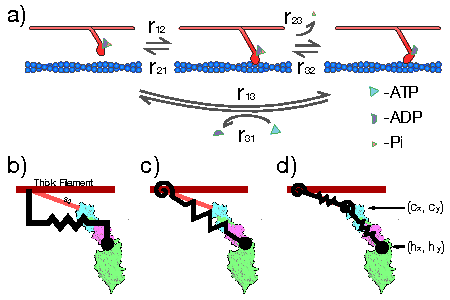
\includegraphics[width=3.2in]{../imgs/Figure1.pdf}
    \label{fig:types}
    \caption{
        Kinetic scheme and crossbridge types under investigation. 
        A) Three state kinetics used in most models and extended here. 
        B) Single spring crossbridge model used in models since \cite{Huxley1957e}. 
        C) Two spring system, consisting of a torsional/angular spring and a linear spring. 
        D) Four spring system using two torsional and two linear springs.}
    \end{center}
\end{figure}

\begin{figure}[p]
    \begin{center}
    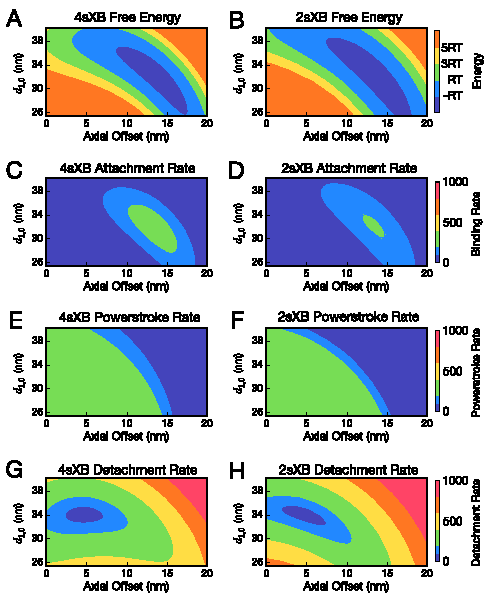
\includegraphics[width=3.2in]{../imgs/Figure2.pdf}
    \label{fig:2s}
    \caption{
        Energy and kinetics of the two spring crossbridge at varying horizontal offsets from a resting location and varying lattice spacings.}
    \end{center}
\end{figure}

\begin{figure}[p]
    \begin{center}
    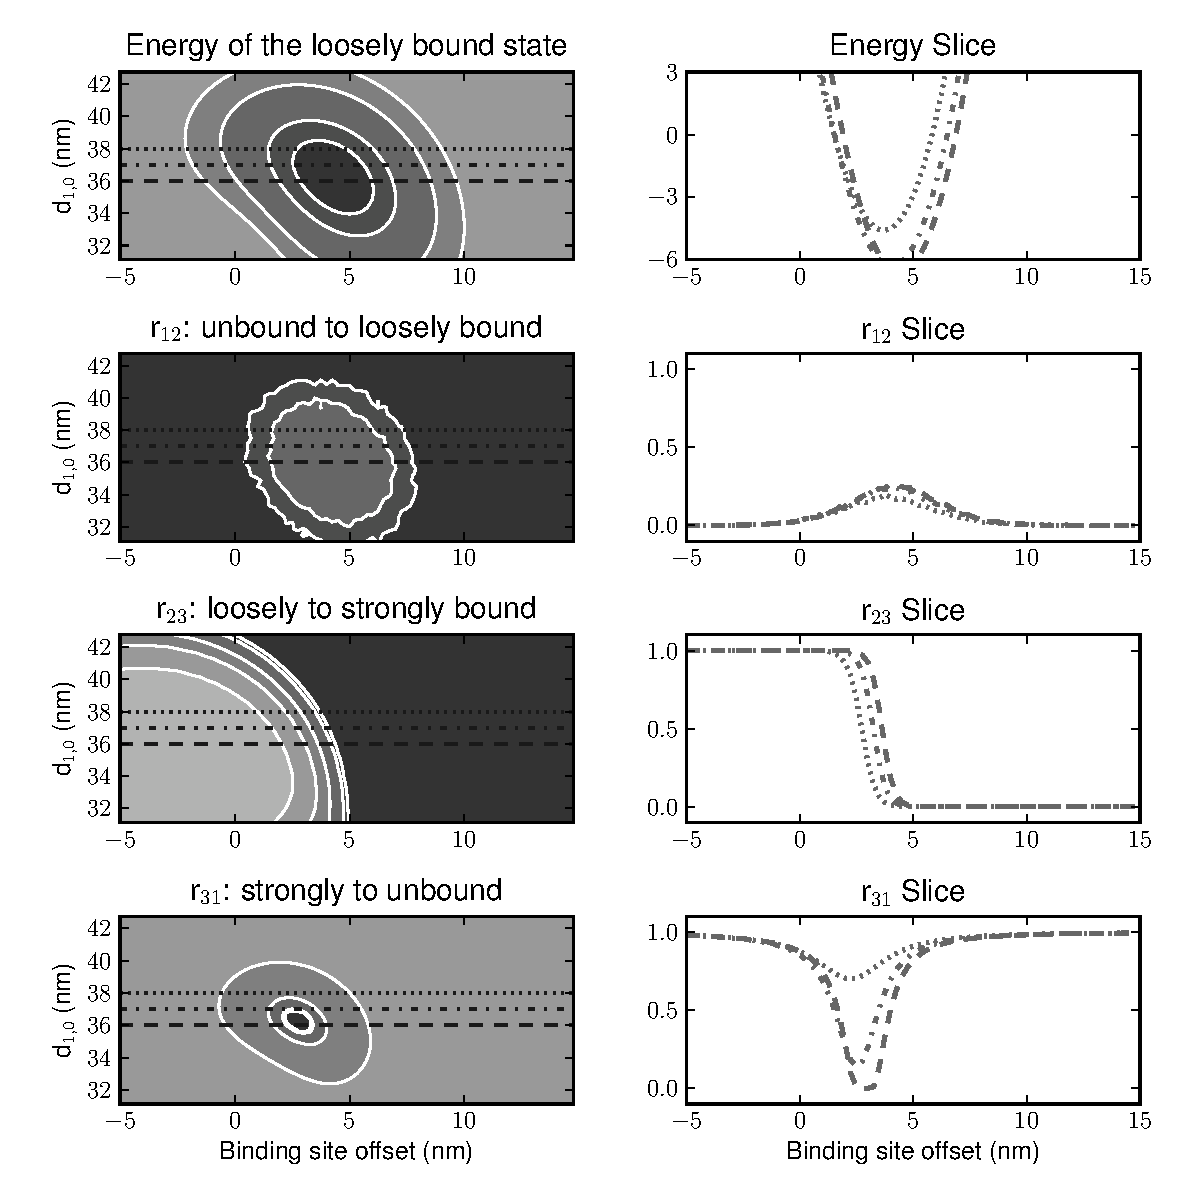
\includegraphics[width=3.2in]{../imgs/Figure3.pdf}
    \label{fig:4s}
    \caption{
        Energy and kinetics of the four spring crossbridge at varying horizontal offsets from a resting location and varying lattice spacings.}
    \end{center}
\end{figure}

\begin{figure}[p]
    \begin{center}
    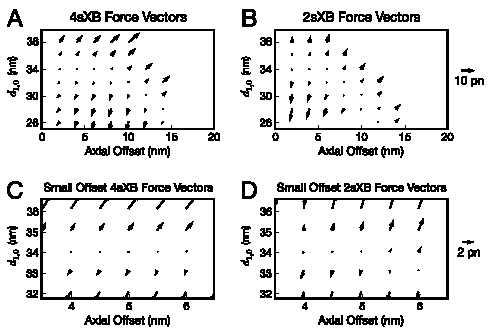
\includegraphics[width=3.2in]{../imgs/Figure4.pdf}
    \label{fig:force}
    \caption{
        Force vectors of the two and four spring crossbridges, and the differences between.}
    \end{center}
\end{figure}

% section figures (end)


% bibliography (fold)
% Bib style requires biophysj.bst be in the document directory
\bibliographystyle{biophysj}
\bibliography{SingleXB}
% bibliography (end)

\end{document}
